\chapter{Hardware}
\label{ch:Hardware}

As aforementioned, we used MIMUs and force plates to gather the raw gait data. In this chapter we will describe in detail the employed hardware, in our case, a device called GaitWatch, developed at the Department of Neurology of the Ludwig-Maximilians University in Munich in conjunction with the Department of Signal Theory, Telematics and Communications of the University of Granada, and a force-measuring plate (Zebris FDM-S). Subsequently, we will elaborate on how the data is arranged in the datasets and carry out the necessary synchronisation of both systems.

\section{GaitWatch}

The GaitWatch device is a MIMU designed to monitor the motion of patients while attached to the body. The system is composed of a set of embedded magnetic and inertial sensors wired to a box containing a microcontroller. This is in charge of collecting data from the embedded box sensors, as well as from the external measurement units, and storing it on a memory card. The several units are placed at the patient's thighs, shanks, arms and trunk as shown in Figure \ref{fig:GaitWatch_placement}. The components of the three different kinds of IMUs are described below:

\begin{figure}
	\centering
	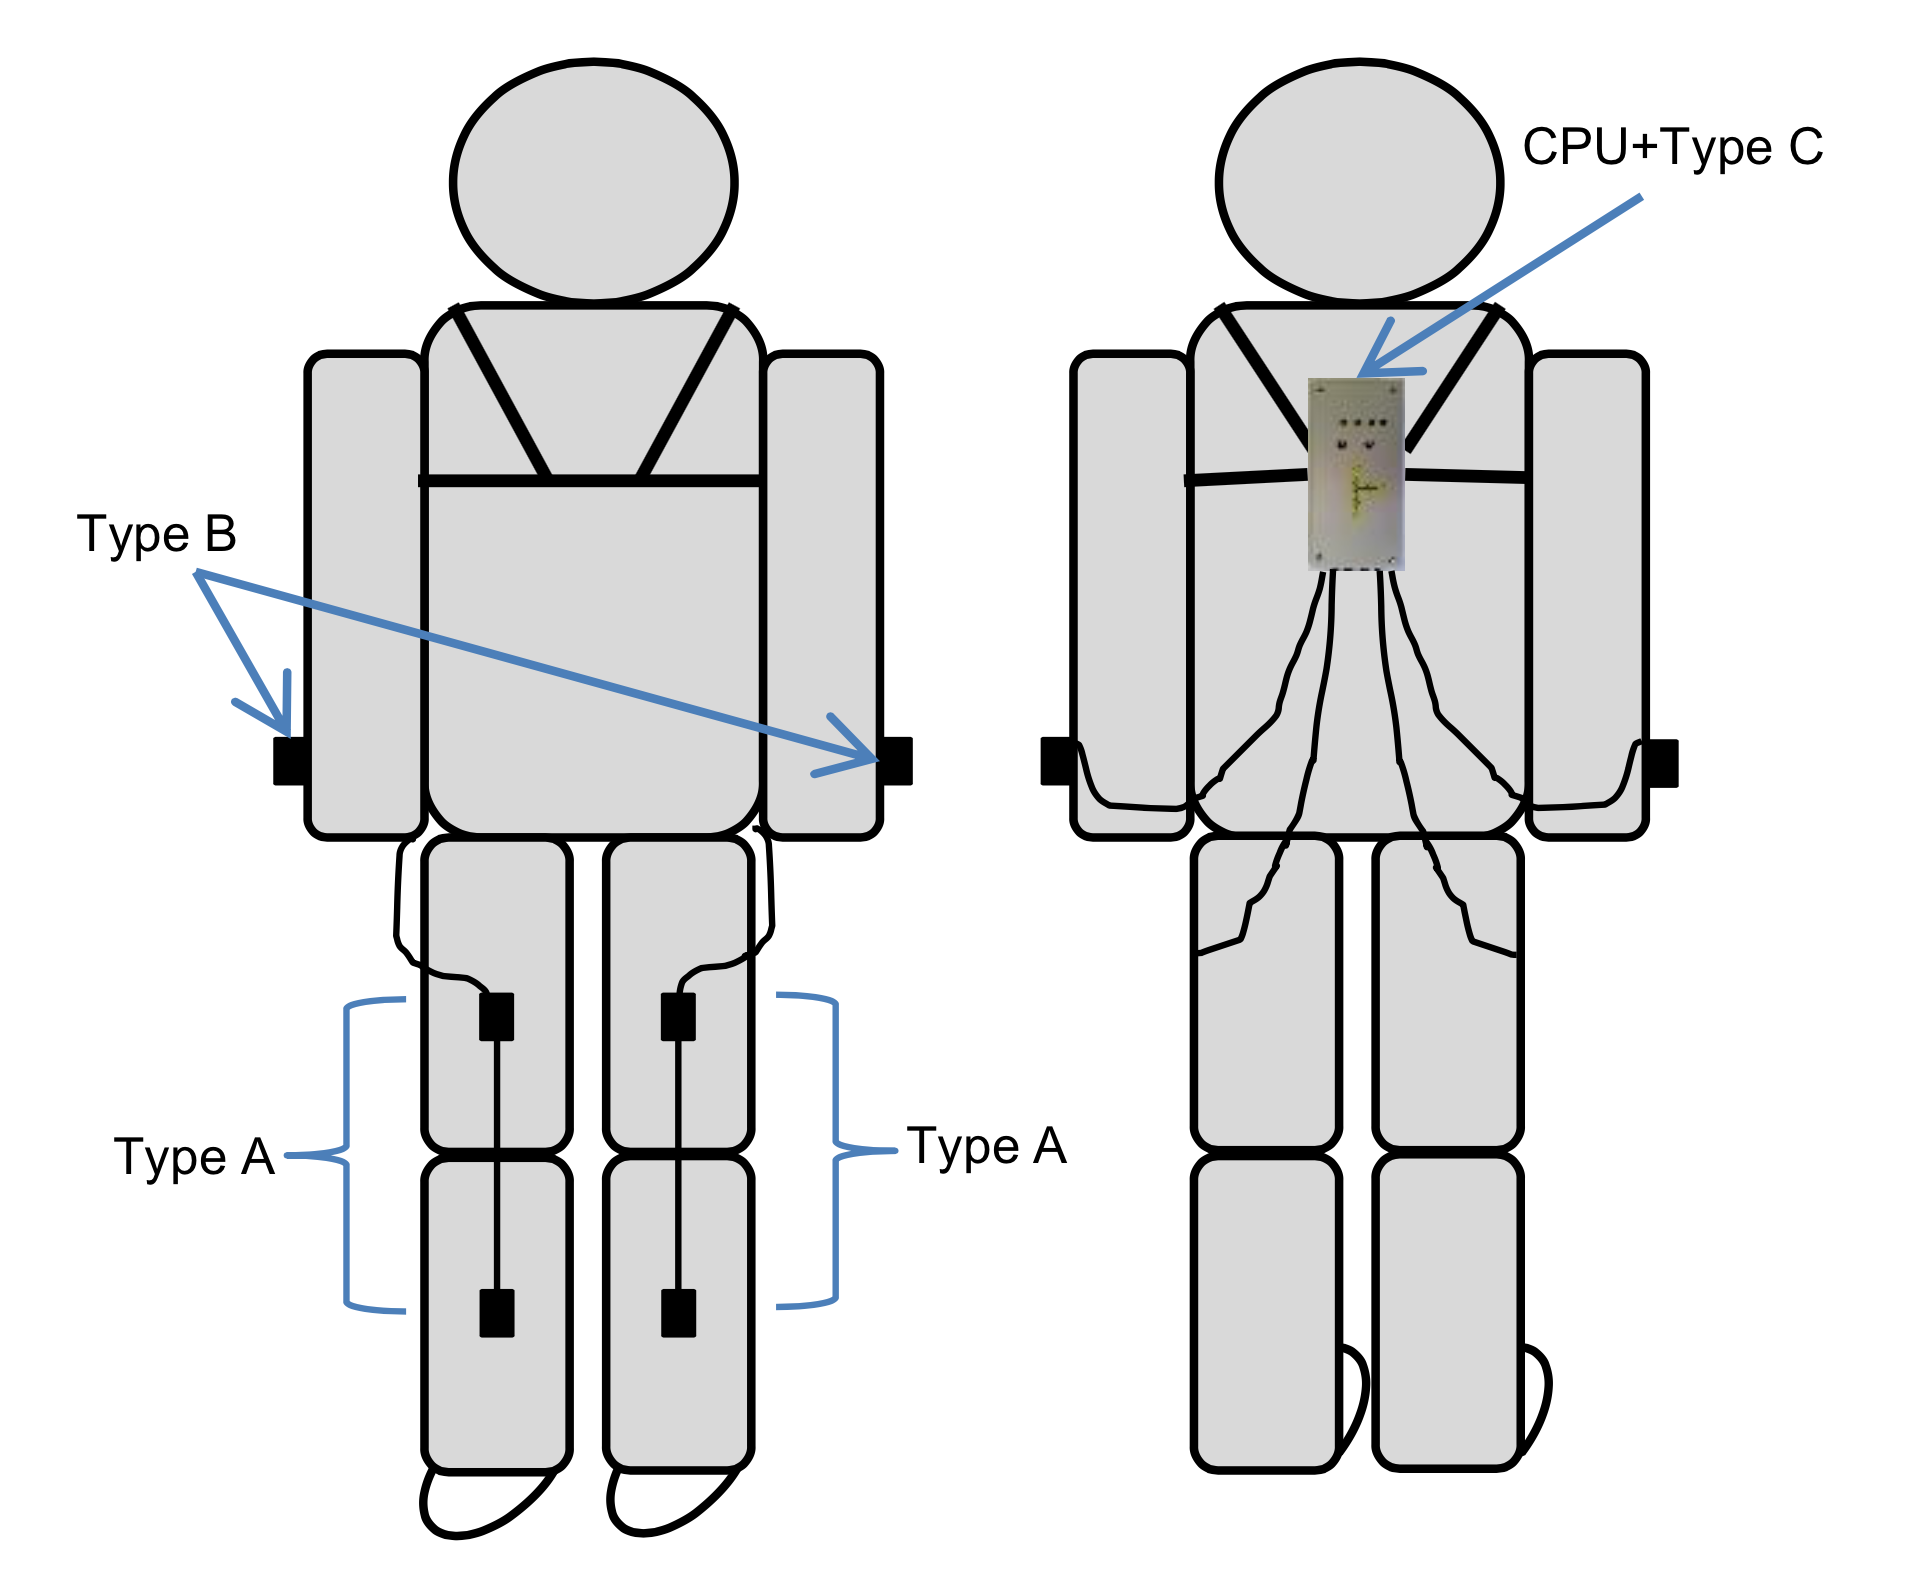
\epsfig{file=images/GaitWatch_placement, width=9cm}
	\caption{Placement of GaitWatch components at the body \cite{olivares_vicente_gaitwatch_2013}.}
	\label{fig:GaitWatch_placement}
\end{figure}

\begin{itemize}

\item \textsc{Type A} (thighs and shanks): 

IMU Analog Combo Board with 5 Degrees of Freedom \cite{IMU5} containing an IDG500 biaxial gyroscope (from which only Y axis is actually used) with a measurement range of ±500°/s \cite{IDG500} and a ±3g triaxial accelerometer, ADXL335 \cite{ADXL335}.

\item \textsc{Type B} (arms):

IDG500 biaxial gyroscope with a measurement range of ±500°/s \cite{IDG500}.

\item \textsc{Type C} (trunk):

ADXL345 triaxial accelerometer with programmable range (±2g/±4g/±8g/±16g) \cite{ADXL345},
IMU3000 triaxial gyroscope with programmable range (±250/±500/±1000/±3000°/s) \cite{IMU3000}, 
Micromag3 triaxial magnetometer with a measurement range of ±11Gauss \cite{MicroMag3}, AL-XAVRB board containing an AVR ATxmega processor \cite{AVRATxmega}.

\end{itemize}


\section{Zebris FDM-S}


\section{Synchronisation}